\chapter{Introduction}

Graph theory is a branch of mathematics concerned with the study of network-like structures called \textit{graphs}.
In this context, a graph consists of a collection of objects (called \textit{vertices}), and any two of these objects may be connected by an \textit{edge}.
Graphs can be used to model all kinds of binary relations. 
For example, the vertices could be a group of people, where two people are connected by an edge whenever they are mutual friends.
In computer science, communication networks are modelled by graphs in which the vertices represent hosts and routers, and the edges represent the communication links between them. 
Navigation systems use graphs to compute the shortest route between two places, and in the natural sciences, graphs can be used, for example, to model chemical structures such as molecules. % (see e.g. \cite{chemicalgraphtheory}).

Leonhard Euler's resolution of the Seven Bridges of Königsberg problem \cite{solutio} is often considered the first mathematical work on graph theory.
Since then, graph theory has evolved into an independent discipline within mathematics.
Over the course of the twentieth century, it has gained particular importance with the rise of computers and the development of theoretical computer science, as many graph-theoretic problems have algorithmic applications and connections to complexity theory.

In addition to combinatorial reasoning, tools from other mathematical disciplines, most notably probability theory, topology, and algebra, have been used to study graphs.
This thesis focuses on spectral graph theory, which investigates the spectral properties of matrices associated with graphs. 
The most natural matrix studied in spectral graph theory is the adjacency matrix. 
For a graph on $n$ vertices, this is an $(n \times n)$ matrix with entries in $\{0, 1\}$, where the entry $(i, j)$ indicates whether there is an edge from the $i$-th vertex to the $j$-th vertex.

In the case of an undirected graph, the adjacency matrix is symmetric. 
Therefore, the spectral theorem from linear algebra implies that all its eigenvalues are real and there exists an orthonormal basis of eigenvectors.
At first glance, it may be surprising that there is a strong interplay between the spectrum and the combinatorial properties of a graph. 
However, upon closer examination, these connections quickly become intuitive, and over the past few decades, a fruitful theoretical framework has been developed.

The simplest of these connections can be illustrated using the example of a $d$-regular graph $G$. 
Suppose that the eigenvalues of the adjacency matrix of $G$ are given by $\lambda_1 \ge \lambda_2 \ge \dots \ge \lambda_n$. 
We will see that:
\begin{itemize}[noitemsep]
    \item The largest eigenvalue satisfies $\lambda_1 = d$.
    \item The graph is connected if and only if $\lambda_1 > \lambda_2$.
    \item The graph is bipartite if and only if $\lambda_1 = -\lambda_n$.
\end{itemize}
Furthermore, a lot of information is provided by the \textit{spectral gap} of $G$, that is, the difference between its largest and second largest eigenvalue.

In addition to revealing interesting structural properties, eigenvalues and eigenvectors of graphs are also useful in their own right:
This can be seen, for example, in Google's PageRank algorithm, which played a key role in the search engine's huge success.
The algorithm ranks the importance of web pages by assigning a numerical weighting to each page.
The idea is that a page which is linked to by more pages should receive a higher weighting, and the higher the weighting of the referencing pages, the higher the weighting of this page (cf. Figure \ref{fig:page-rank}).
The PageRank algorithm achieves this by assigning to each page the corresponding entry of the Perron eigenvector (see Section \ref{section:perron-frobenius}) of an associated matrix of the World Wide Web graph. 
The vertices of the underlying directed graph are web pages $P_1, \dots, P_n$, with an edge from $P_i$ to $P_j$ whenever $P_i$ contains a hyperlink referencing $P_j$.
More details on PageRank can be found in \cite{thelinearalgebrabehindgoogle}.

\begin{figure}[h]
    \centering
    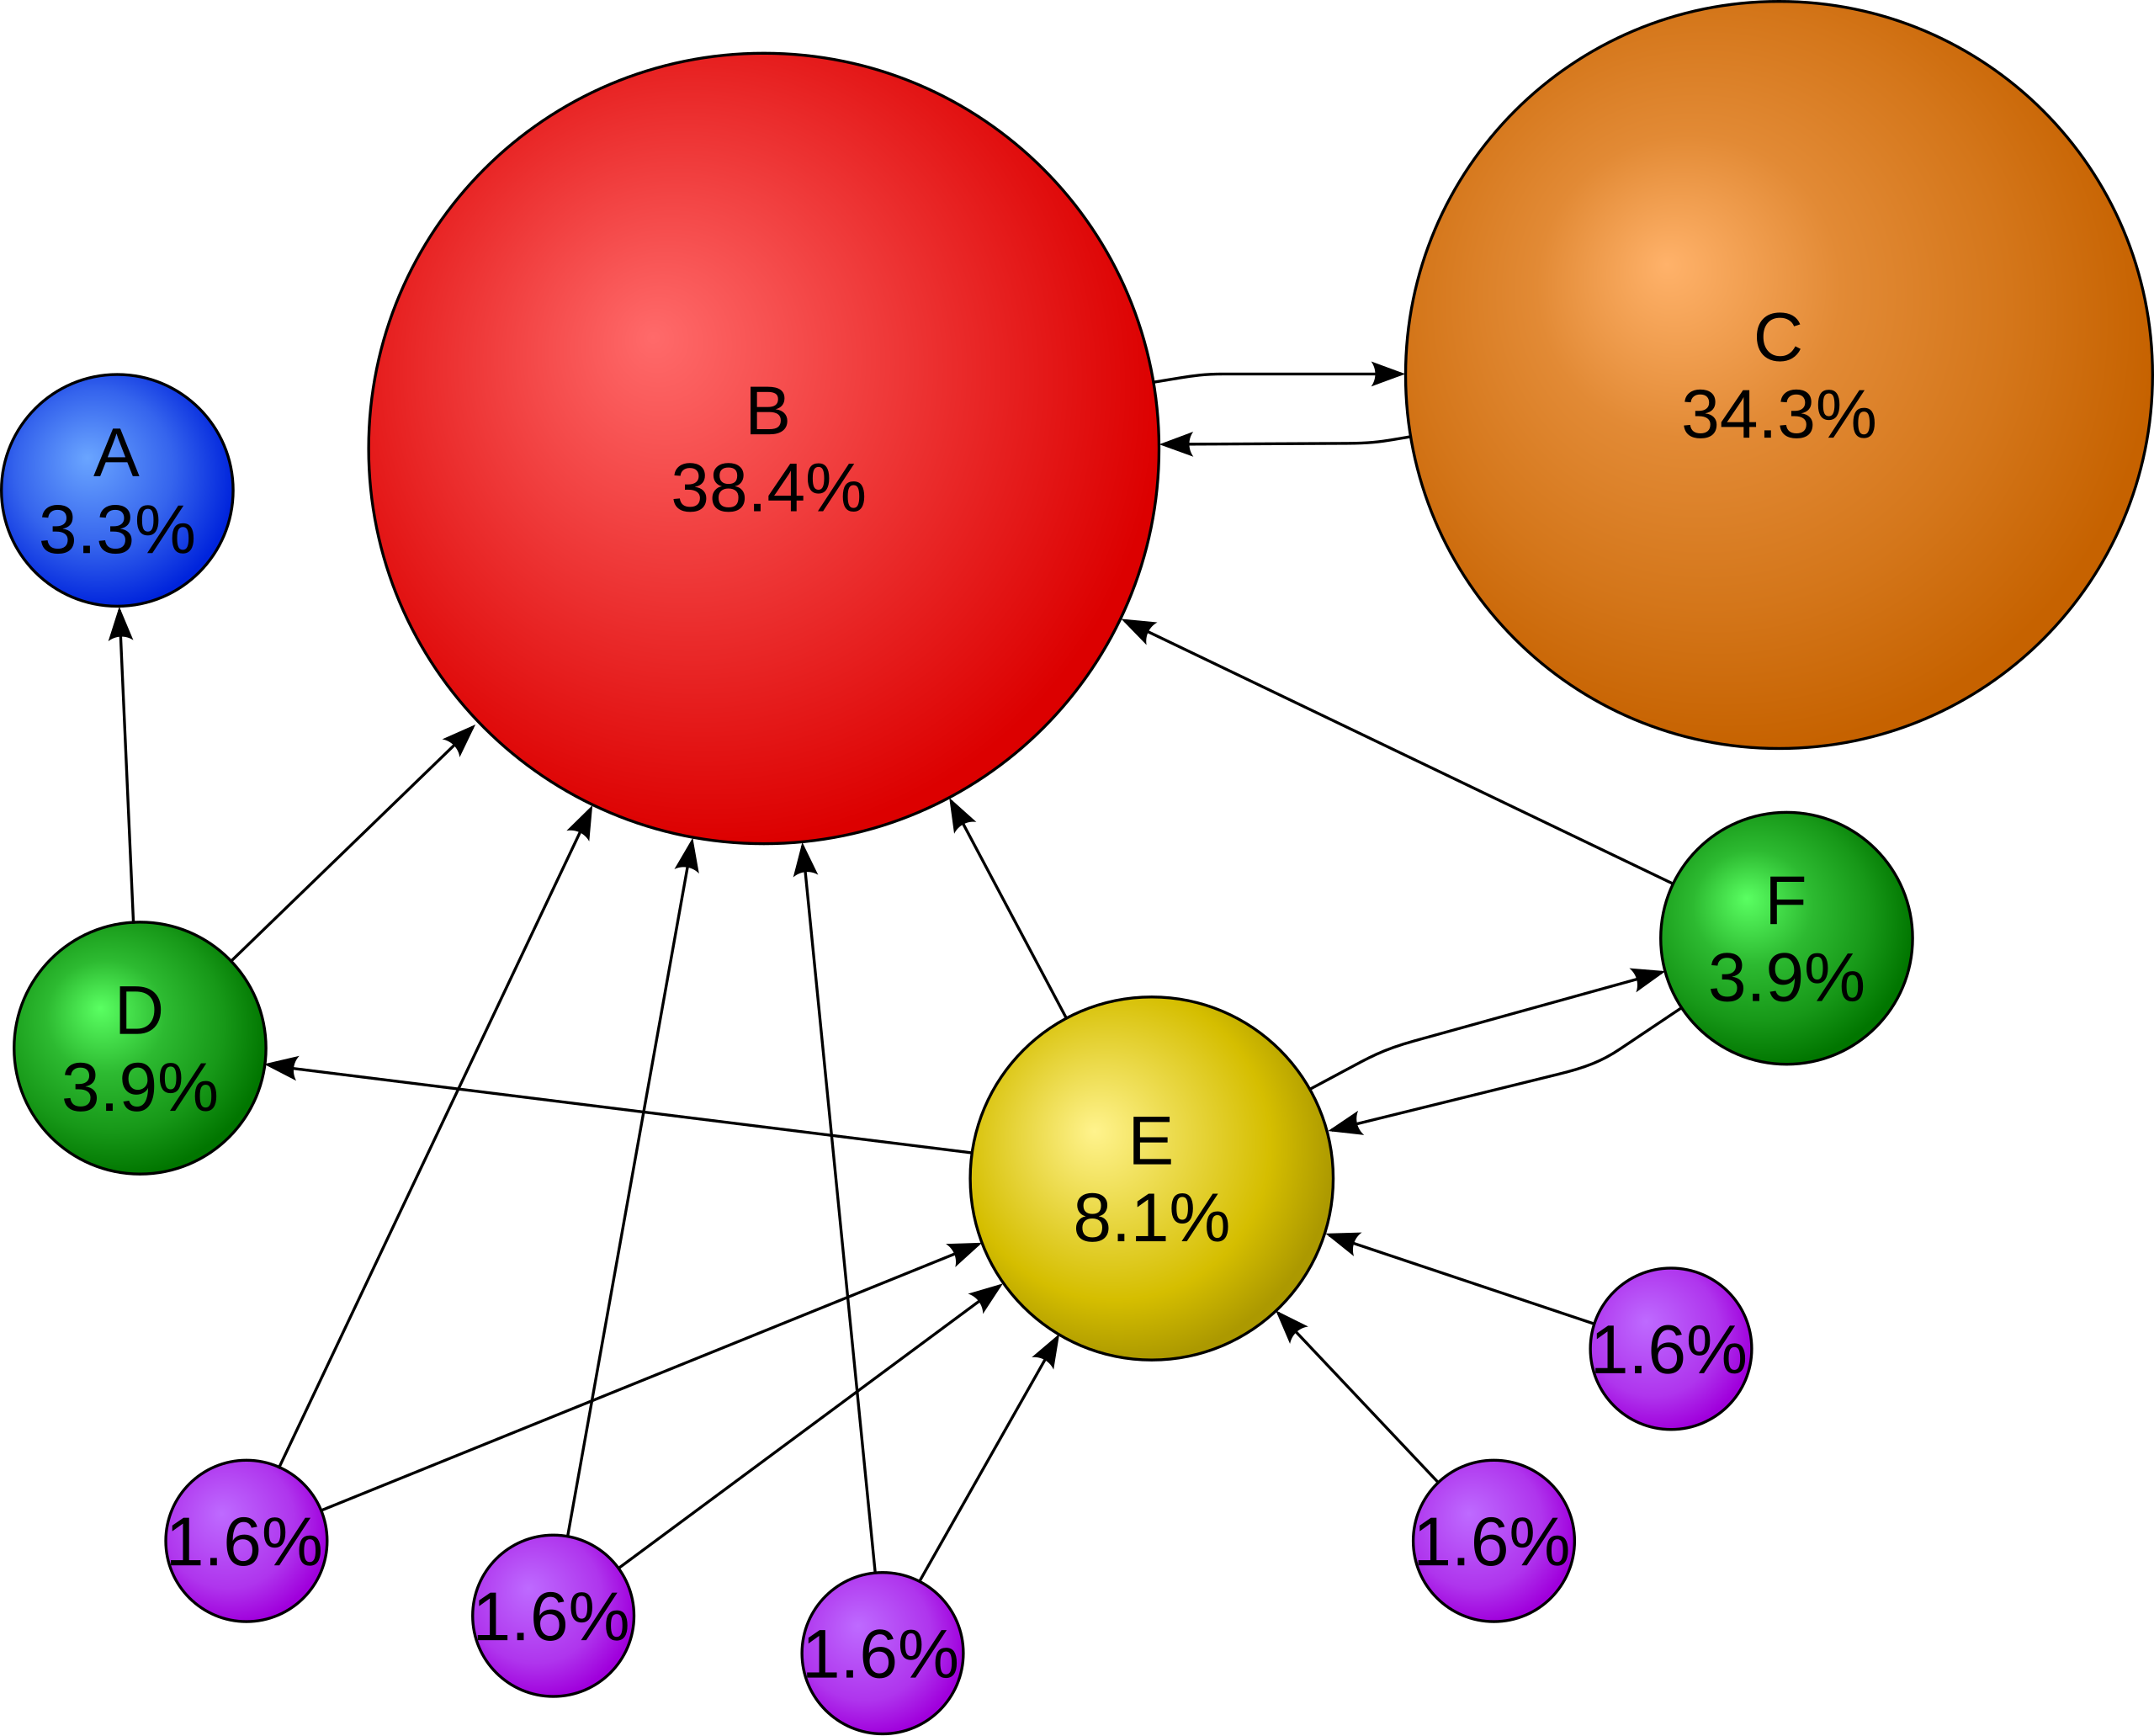
\includegraphics[width=0.6\linewidth]{images/PageRanks-Example.svg.png}
    \caption{The PageRank algorithm applied to a small graph. Taken \mbox{from \cite{wikimedia-pagerank}.}}
    \label{fig:page-rank}
\end{figure}

Furthermore, spectral techniques have been used to give proofs for seemingly purely combinatorial problems such as the Erd\H os--Ko--Rado theorem (see Section \ref{section:hoffman-bound}) or the Sensitivity Conjecture (see Section \ref{section:sensitivity}).

\section{Thesis outline}
The goal of this thesis is twofold.
First, we provide an overview of the foundations of spectral graph theory and present some classical results.
Secondly, we give an in-depth review of two disparate recent research results that showcase the connections of spectral graph theory to geometry and computer science.

In Chapter 2, we start by defining the basic graph-theoretic concepts encountered throughout this thesis, as well as the most prominent matrices that arise in spectral graph theory.
Then, we introduce some useful tools from linear algebra, such as the Perron--Frobenius theorem and the Cauchy interlacing theorem, and apply them to obtain elementary information about the spectrum of the adjacency matrix of a graph.

Chapter 3 presents some classical results from spectral graph theory that relate the combinatorial properties of a graph to its spectrum. 
The first part of this chapter treats the concept of graph expansion and Cheeger's inequality.
Roughly speaking, an expander graph is a (usually sparse) graph with very good connectivity properties, so that one cannot disconnect two large parts of the graph by removing a small number of edges. 
Cheeger's inequality, one of the most important results of spectral graph theory, states that a large spectral gap is qualitatively equivalent to good expansion properties.

In the remainder of this chapter, we cover Hoffman's bound and the Expander mixing lemma.
The former result provides a bound on the independence number in terms of the smallest eigenvalue of a graph, while the latter relates the spectrum of a graph to a particular pseudorandomness property: 
It asserts that the edges of certain regular graphs are "spread out" in the sense that their edge distribution resembles that of a random graph.

Chapters 4 and 5 deal with applications of spectral graph theory to other subfields of mathematics.
In addition to providing insight into specific research topics, both chapters are meant to demonstrate how spectral methods can be used to give surprisingly elegant proofs for problems that have little connection to graph theory at first sight. 
The following two sections provide a first overview of these applications.

Chapter 6 concludes the thesis and hints at possible sources for further reading.

\section{An application in geometry}

In Chapter 4, we discuss the resolution of a long-standing geometric problem concerning equiangular lines. 
Even though the connection to graph theory is far from obvious, the study of equiangular lines is named one of the founding problems of spectral graph theory in the classic textbook Algebraic Graph Theory \cite{godsilroyle} by Godsil and Royle.
For $\alpha \in (0, 1)$, let $N_\alpha (d)$ denote the maximum number of lines with pairwise angle $\arccos \alpha$ in $\R^d$. 
The problem of determining $N_\alpha (d)$ for a fixed $\alpha$ and large dimensions $d$ dates back to 1973, when Lemmens and Seidel \cite{lemmensseidel} introduced the quantity.
In a recent work, Jiang, Tidor, Yao, Zhang, and Zhao \cite{equiangular} solved this problem using tools of spectral graph theory. 
For the case where $\alpha = 1 / (2k - 1)$ for some integer $k \ge 2$ and $d$ is sufficiently large, their main result states that $N_\alpha(d) = \lfloor k (d - 1) / (k - 1) \rfloor$.

A major ingredient in their proof is a novel result in spectral graph theory that gives insight into the distribution of the eigenvalues of a graph:
They showed that the second largest eigenvalue of a connected $n$-vertex graph with bounded maximum degree has multiplicity at most $O(n / \log \log n)$.\footnote{The largest one has multiplicity $1$.}
To the best of our knowledge, this is the first result of this form for general graphs.
Currently, there is still a significant gap between this bound and the best-known lower bound constructions, which achieve a second eigenvalue multiplicity of $n^{1 /2 - o(1)}$.
This led the authors of \cite{equiangular} to ask whether their bound can be improved.
Addressing this question, we end Chapter 4 by establishing stronger bounds for the special case of graph classes with small balanced separators.

\section{An application in computer science}
Chapter 5 presents the recent breakthrough proof of the Sensitivity Conjecture, which has stood as one of the most prominent open problems in theoretical computer science for almost three decades.
The conjecture concerns the relationship between two different complexity measures for Boolean functions, \textit{sensitivity} and \textit{block sensitivity}. 
Posed by Nisan and Szegedy \cite{nisanszegedy} in 1992, the Sensitivity Conjecture states that these complexity measures are polynomially related (and hence equivalent in the sense of complexity theory).
Although numerous researchers had previously worked on the problem, very little progress was made until 2019, when Huang \cite{sensitivity} finally published a proof of the conjecture. 
His work builds upon a reduction due to Gotsman and Linial \cite{gotsmanlinial}, according to which it suffices to show that every induced subgraph of the $n$-dimensional hypercube on more than half of the vertices has maximum degree at \mbox{least $\sqrt{n}$}.
Huang's proof uses techniques from spectral graph theory and is notable for its simplicity and succinctness.

\paragraph{Notation and preliminaries.}
By $\N$ we denote the set of natural numbers starting from $1$; to include 0 we write $\N_0$. 
By $[n]$ we denote the set $\{1, 2, \dots, n\}$. 
Given a set $X$ and $k \le |X|$, we write $\binom{X}{k}$ for the set of all $k$-element subsets of $X$.

The $(n \times n)$-identity matrix is denoted by $I_n$. 
Similarly, we write $J_{m,n}$ for the $(m \times n)$ all-ones matrix, or $J_n$ for a square matrix.
If the size can be inferred from the context, we will usually drop the subscript.

We view $\R^n$ together with the Euclidean norm and scalar product throughout.
That means, for vectors $\bm{x}, \bm{y} \in \R^n$, we write $\langle \bm{x}, \bm{y} \rangle := \bm{x}^T \bm{y}$, and $\| \bm{x} \|\; := \sqrt{\langle \bm{x}, \bm{x} \rangle}$.
Vectors are denoted in bold as $\bm{x}, \bm{y}, \bm{v}, \bm{w}$ etc. to distinguish them from graph vertices $x, y, v, w, \dots$, which are typically named with the same letters.
It may occur that the vertices of a graph are vectors themselves.
In this case, we only use bold notation when we want to emphasise this feature.
The all-ones vector is denoted by $\bm{1}$, the $j$-th unit vector is denoted \mbox{by $\bm{e}_j$}.

All logarithms are taken to base $e$, unless denoted otherwise by a subscript.

The reader is assumed to be familiar with elementary linear algebra, especially concepts such as eigenvalues and orthonormal bases.
Standard results that can be found in most undergraduate textbooks, such as the rank-nullity theorem or the spectral theorem, will be used without further explanation. 
All necessary graph-theoretic notions, on the other hand, will be defined in the thesis.
